%  LaTeX support: latex@mdpi.com 
%  For support, please attach all files needed for compiling as well as the log file, and specify your operating system, LaTeX version, and LaTeX editor.

%=================================================================
\documentclass[life,article,submit,pdftex,moreauthors]{Definitions/mdpi} 

%% The amssymb package provides various useful mathematical symbols
\usepackage{amssymb}
%% The amsmath package provides various useful equation environments.
\usepackage{amsmath}
%% The amsthm package provides extended theorem environments
%% \usepackage{amsthm}
\usepackage{array}
\usepackage{tabularx}
\usepackage{booktabs}
\usepackage{algorithm}
\usepackage{algorithmic}

%=================================================================
% MDPI internal commands - do not modify
\firstpage{1} 
\makeatletter 
\setcounter{page}{\@firstpage} 
\makeatother
\pubvolume{1}
\issuenum{1}
\articlenumber{0}
\pubyear{2025}
\copyrightyear{2025}
%\externaleditor{Academic Editor: Firstname Lastname}
\datereceived{ } 
\daterevised{ } % Comment out if no revised date
\dateaccepted{ } 
\datepublished{ } 
%\datecorrected{} % For corrected papers: "Corrected: XXX" date in the original paper.
%\dateretracted{} % For corrected papers: "Retracted: XXX" date in the original paper.
\hreflink{https://doi.org/} % If needed use \linebreak
%\doinum{}
%\pdfoutput=1 % Uncommented for upload to arXiv.org
%\CorrStatement{yes}  % For updates

%=================================================================
% Full title of the paper (Capitalized)
\Title{Stability-Driven Assembly: A Natural Genetic Algorithm and Pathway to Evolution}


% MDPI internal command: Title for citation in the left column
\TitleCitation{Stability-Driven Assembly: A Natural Genetic Algorithm and Pathway to Evolution}

% Author Orchid ID: enter ID or remove command
\newcommand{\orcidauthorA}{0009-0007-7122-0317} % Add \orcidA{} behind the author's name

% Authors, for the paper (add full first names)
\Author{Dan Adler $^{1}$\orcidA{}}

% MDPI internal command: Authors, for metadata in PDF
\AuthorNames{Dan Adler}

% Affiliations / Addresses
\address{%
$^{1}$ \quad dan@danadler.com}

%=================================================================
% Abstract (Do not insert blank lines, i.e. \\) 
\abstract{
The emergence of evolutionary dynamics before the existence of dedicated replicators remains a central paradox in origins-of-life research: replication requires replicators, yet such machinery presupposes prior replication. We propose \textit{Stability-Driven Assembly} (SDA) as a natural resolution. SDA operates through four simple rules: stochastic creation of assemblies, persistence bias favoring stable motifs, expiration of unstable species, and replenishment of inputs. These dynamics are formally isomorphic to a genetic algorithm: variation arises from recombination and mutation, while persistence functions as fitness. Stable substructures act as schemata, preserved across generations, as illustrated in our simulation by the persistence of functional groups in organic chemistry. Unlike pre-specified target searches such as Dawkins’ “weasel” example, SDA is an open-ended evolutionary process that generates novel information and naturally favors stability. Iterating this loop allows chemical systems to perform an evolutionary search without external programming, suggesting a plausible pathway from chemistry to Darwinian evolution. More broadly, SDA highlights how persistence imbalances give rise to apparent teleology, why life-like order is inevitable in localized, non-equilibrium pockets that accumulate stability while exporting entropy, and why biospheres elsewhere may be universal in process yet diverse in outcome. Finally, we explore implications for computation beyond Turing, astrobiology, and biological longevity, positioning SDA as a unifying principle connecting chemistry, computation, and evolution.
}

% Keywords
\keyword{Stability-Driven Assembly; Genetic Algorithms; Emergent computation; Information dynamics; Origins of life; Astrobiology; Teleology; Persistence bias; Open-ended evolution}

%=================================================================
\begin{document}

\section{Introduction}

\section{Stability-Driven Assembly (SDA)}

A Stability-Driven Assembly (SDA) \cite{adler_sda} system is formally defined as a tuple $(E, P, S, R, I)$ where:
\begin{itemize}
   \item $E = \{e_1, e_2, \ldots, e_n\}$ is a finite set of base elements
   \item $P$ is the set of all possible patterns formed by concatenating elements from $E$ and existing patterns
   \item $S: P \rightarrow \mathbb{Z}^{+}$ is a stability function mapping each pattern to a non-negative integer representing its lifetime
   \item $R: E \rightarrow \mathbb{Z}^{+}$ is a replenishment function specifying how many copies of each base element are added per generation
   \item $I \in \mathbb{Z}^{+}$ is the number of interactions allowed per generation
\end{itemize}

The pattern interaction operation, denoted by $\oplus$, is defined as a string concatenation. When patterns $p_1$ and $p_2$ interact, they form a pattern $p_1 \oplus p_2$.

\begin{algorithm}[H]
\caption{SDA System Simulation}
\footnotesize
\begin{algorithmic}[1]
\REQUIRE Base elements $E$, stability function $S$, replenishment rates $R$, interaction count $I$, generations $T$
\ENSURE Pattern population evolution over $T$ generations
\STATE Initialize population with base elements
\FOR{$t = 1$ to $T$}
   \STATE Remove expired patterns
   \STATE Add $R(e)$ copies of each element $e \in E$ to population
   \FOR{$i = 1$ to $I$}
       \STATE Select patterns $p_1$, $p_2$ randomly from population
       \STATE Form $p_{new} = p_1 \oplus p_2$
       \STATE Set expiration time for $p_{new}$ to $t + S(p_{new})$
       \STATE Add $p_{new}$ to population
   \ENDFOR
\ENDFOR
\end{algorithmic}
\end{algorithm}


The probability of selecting a pattern $p$ for interaction is proportional to its frequency in the population. This creates a feedback mechanism: patterns with higher stability persist longer, becoming more abundant, which increases their probability of participating in interactions.

The original SDA formulation emphasizes string concatenation as the sole pattern-forming operation. In what follows, we generalize the interaction to a recombination operator with an optional mutation step, and then examine whether the core properties of SDA are preserved under this extension. Instead of:
\[
p_{\text{new}} = p_1 \oplus p_2,
\]
we use a recombination of the two patterns:
\[
p_{\text{new}} = \mathrm{Recombine}(p_1,p_2),
\]
optionally followed by a \emph{single–site mutation} applied with probability $\mu$:
\[
p_{\text{new}} =
\begin{cases}
\mathrm{Mutate}(p_{\text{new}}) & \text{with probability } \mu,\\
p_{\text{new}} & \text{with probability } 1-\mu.
\end{cases}
\]
This change does not alter the selection mechanism: persistence 
$S(p)$ still determines
residence time and thus induces roulette–wheel selection in expectation.

\subsection{Simulation Results}

We begin by comparing the final pattern distributions produced by the original SDA with concatenation and the generalized SDA/GA with recombination. Both systems show strong deviation from the unconstrained case: instead of a uniform spread of short strings, high-stability motifs dominate the population. In the SDA system, concatenation drives the emergence of long repeated motifs such as \texttt{ABCABA}, which concentrate much of the probability mass. In the recombination-based GA variant, the same dominant motifs appear, but the distribution shows a heavier tail: many low-frequency variants persist alongside the stable core (Figures~\ref{fig:concat-patterns},~\ref{fig:ga-patterns}). This broader spectrum reflects recombination’s ability to continuously inject mosaic offspring and maintain a pool of rare types, whereas pure concatenation channels more strongly into layered repeats.

\begin{figure}[H]
    \centering
    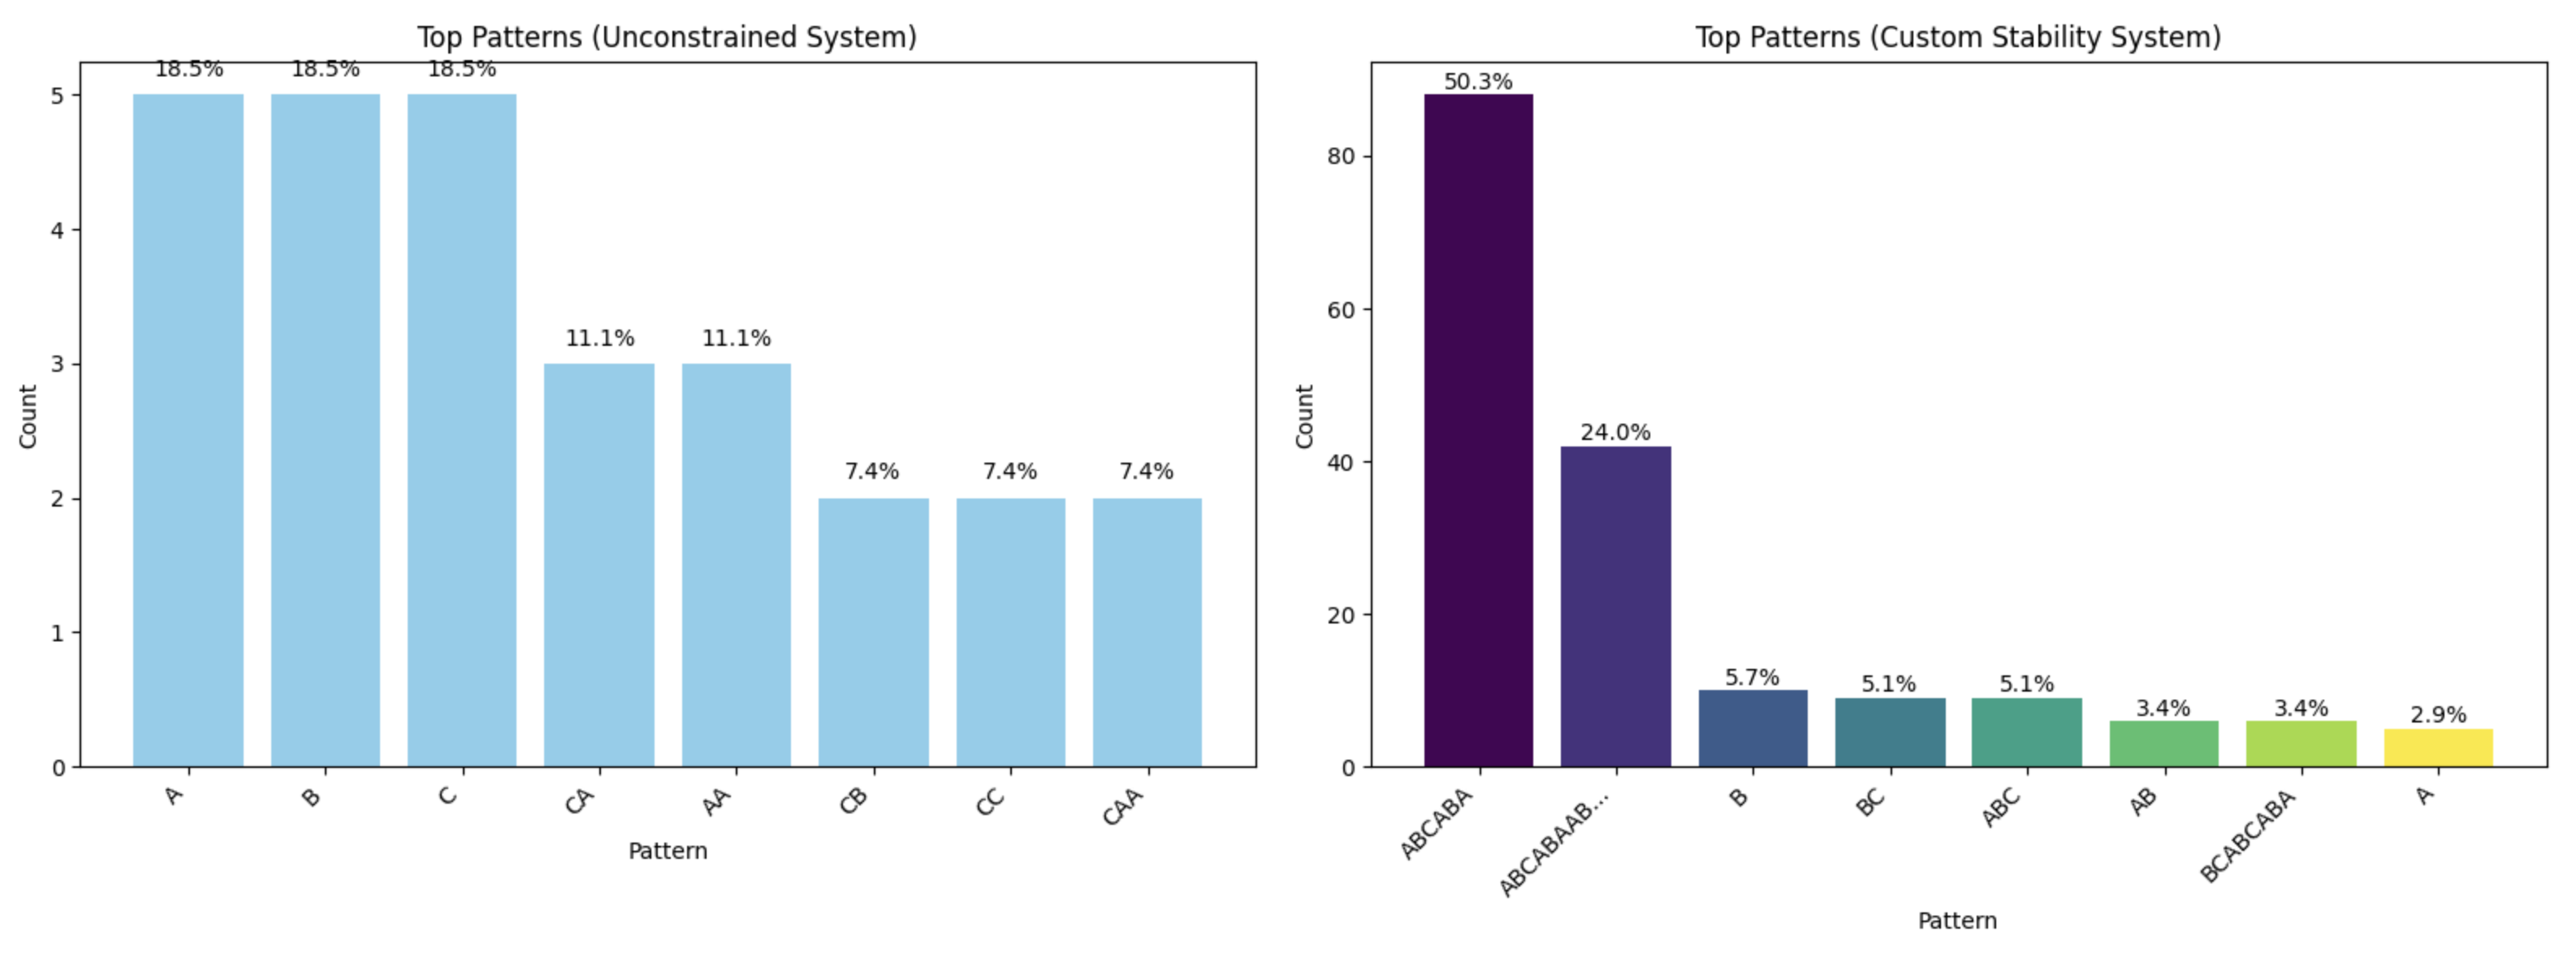
\includegraphics[width=1\textwidth]{SDA-concat-patterns.png}
    \caption{Pattern distribution in the SDA system with concatenation. A small set of high-stability motifs dominate the population, while other patterns are nearly absent.}
    \label{fig:concat-patterns}
\end{figure}

\begin{figure}[H]
    \centering
    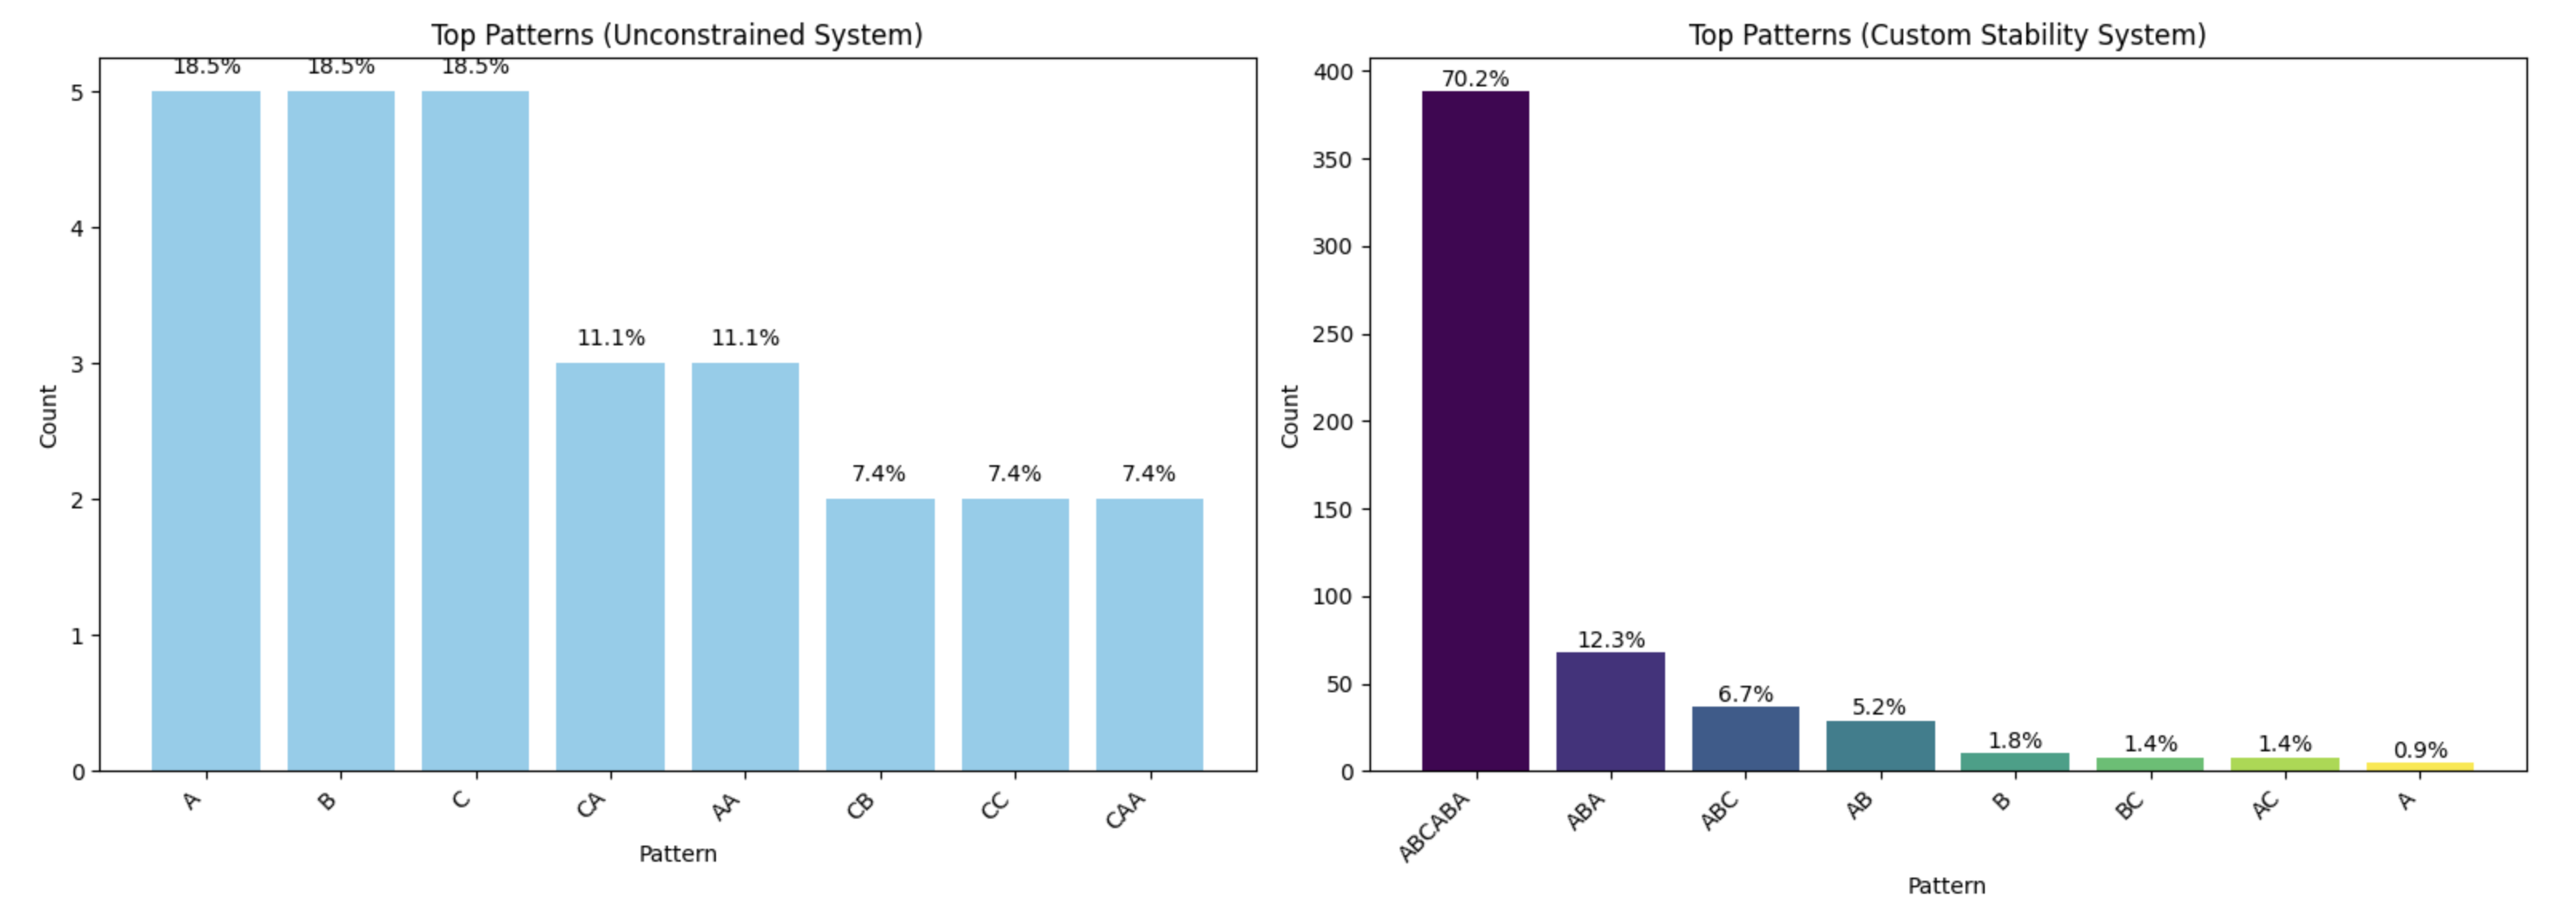
\includegraphics[width=1\textwidth]{SDA-GA-patterns.png}
    \caption{Pattern distribution in the generalized SDA/GA system with recombination. Stable motifs dominate as in the pure SDA case, but a broader tail of low-frequency variants persists due to recombination.}
    \label{fig:ga-patterns}
\end{figure}

Turning to entropy dynamics, both systems show clear reduction in Shannon entropy ($H(P_t) = - \sum_{p \in P} P_t(p) \log_2 P_t(p)$) of
the pattern distribution at generation t measured in bits relative to the unconstrained baseline, confirming the emergence of order and the presence of selection pressure (Figures~\ref{fig:concat-entropy},~\ref{fig:ga-entropy}). Importantly, this occurs without any explicit fitness-proportional selection rule in the algorithm: roulette-wheel selection emerges intrinsically from persistence, since patterns with longer lifetimes are overrepresented and thus more likely to be sampled for further interactions.

In the concatenation-based SDA, while the average entropy goes down from $\sim6$ bits to $\sim4$ bits, its trajectories often exhibit oscillations. These arise because concatenation tends to build large, synchronized cohorts of similar long motifs, which expire at nearly the same time. When such a cohort collapses, replenished base elements briefly increase diversity and entropy before new dominant motifs emerge, creating a characteristic boom–bust cycle. In contrast, in the recombination-based SDA/GA, entropy decreases more smoothly to $\sim3$ bits without oscillations. Recombination produces mosaic offspring with staggered lifetimes, desynchronizing expirations and damping collective turnover. The result is a more monotonic entropy collapse toward a skewed distribution anchored by stable motifs.

\begin{figure}[H]
    \centering
    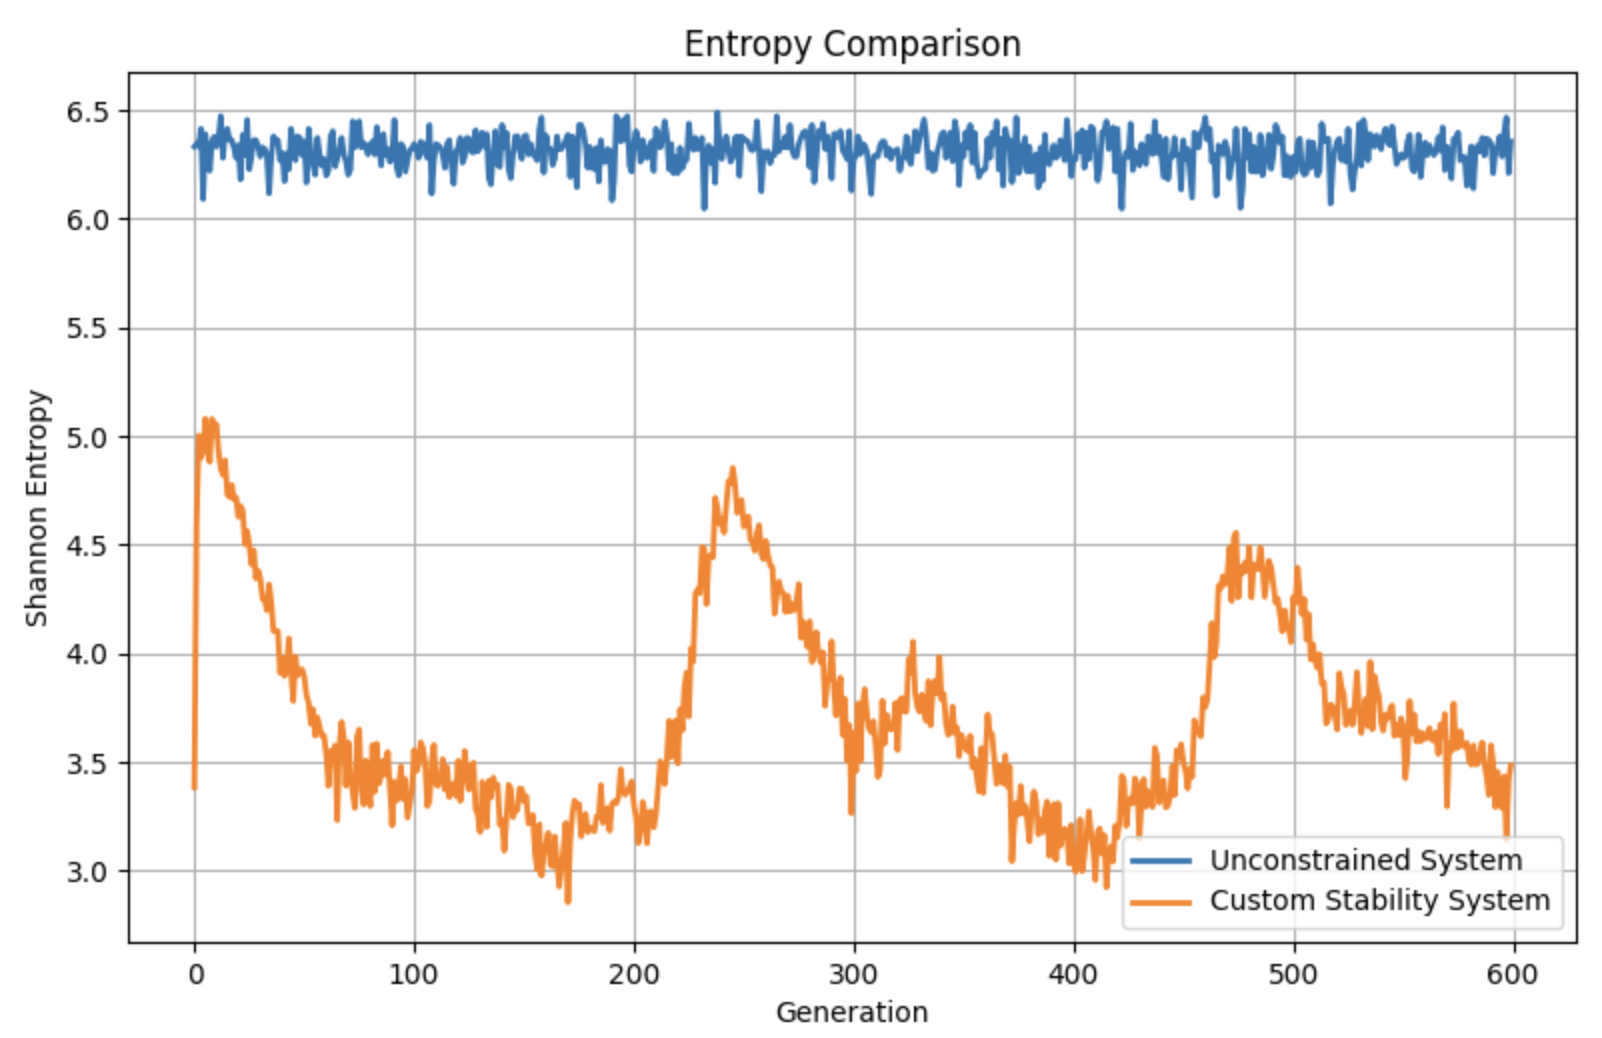
\includegraphics[width=0.8\textwidth]{SDA-concat-entropy.png}
    \caption{Entropy dynamics in the concatenation-based SDA system. Entropy decreases overall but exhibits oscillatory boom–bust cycles due to synchronized expiration of long motifs.}
    \label{fig:concat-entropy}
\end{figure}

\begin{figure}[H]
    \centering
    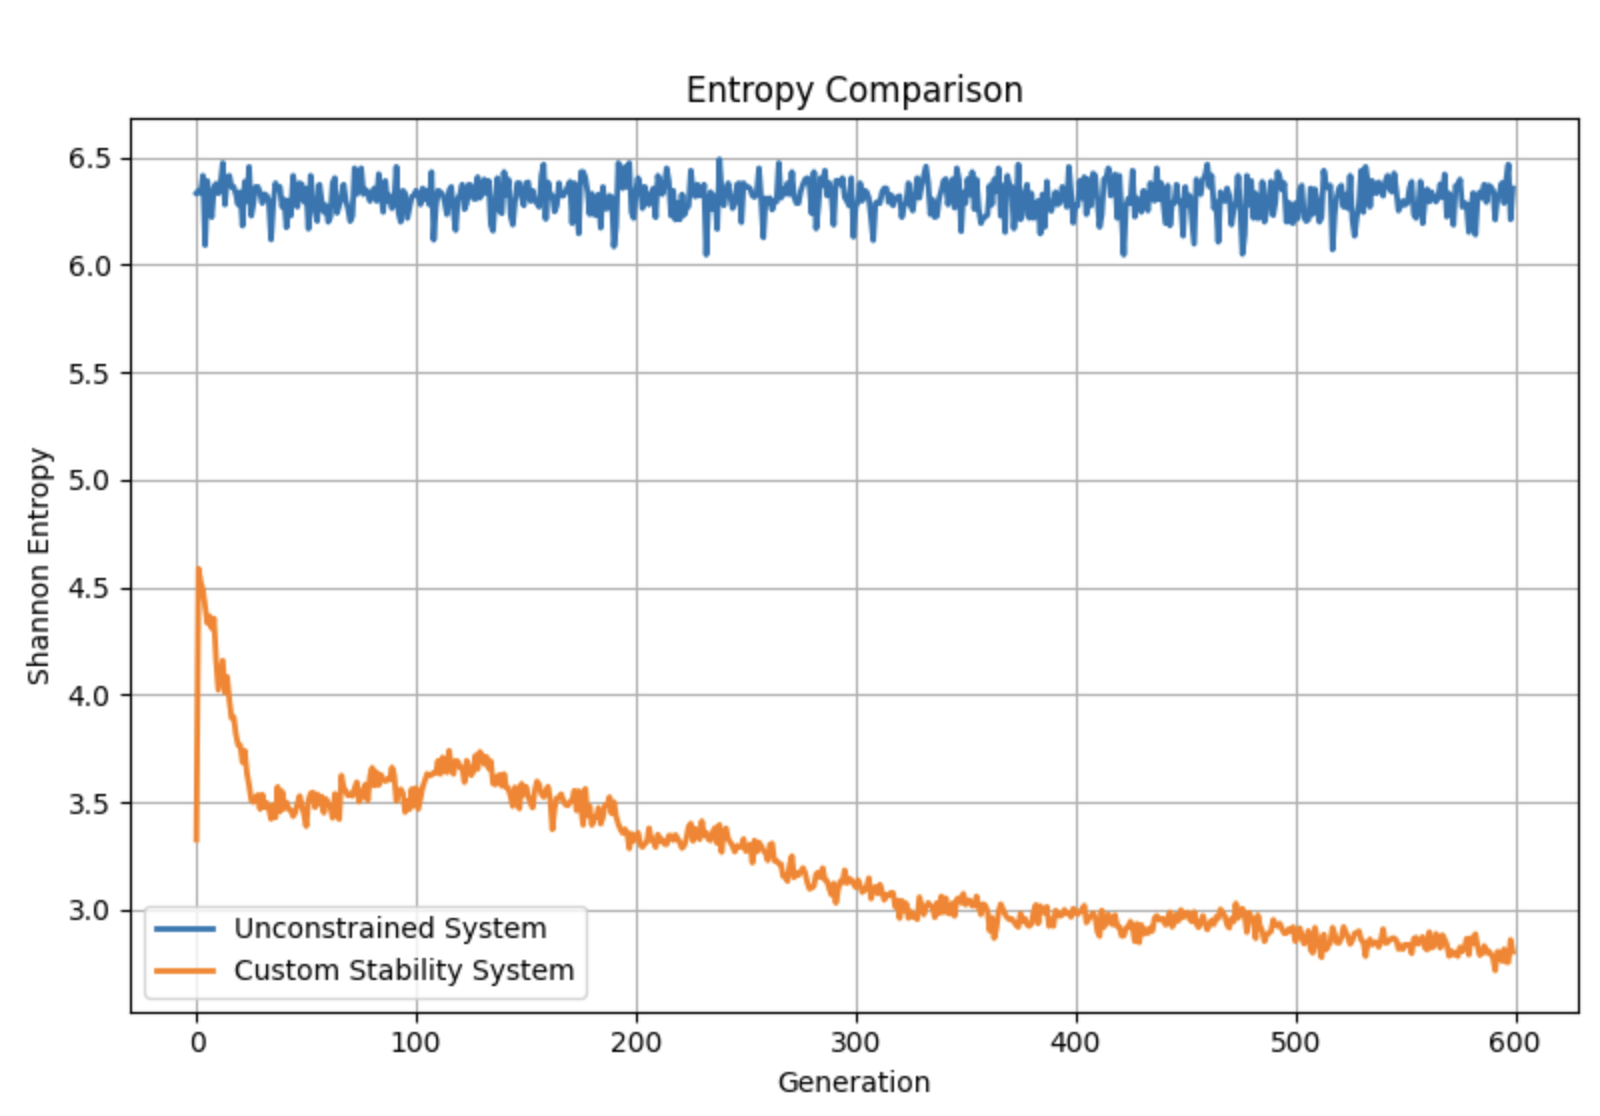
\includegraphics[width=0.8\textwidth]{SDA-GA-entropy.png}
    \caption{Entropy dynamics in the recombination-based SDA/GA system. Entropy decreases smoothly without oscillations, as recombination desynchronizes expirations.}
    \label{fig:ga-entropy}
\end{figure}

Together, these results demonstrate that stability-driven assembly robustly yields emergent selection pressure and entropy reduction under both concatenation and recombination operators. The choice of interaction operator primarily shapes the dynamical form of convergence: oscillatory cycles under concatenation versus smooth decline under recombination.

\begin{figure}[H]
    \centering
    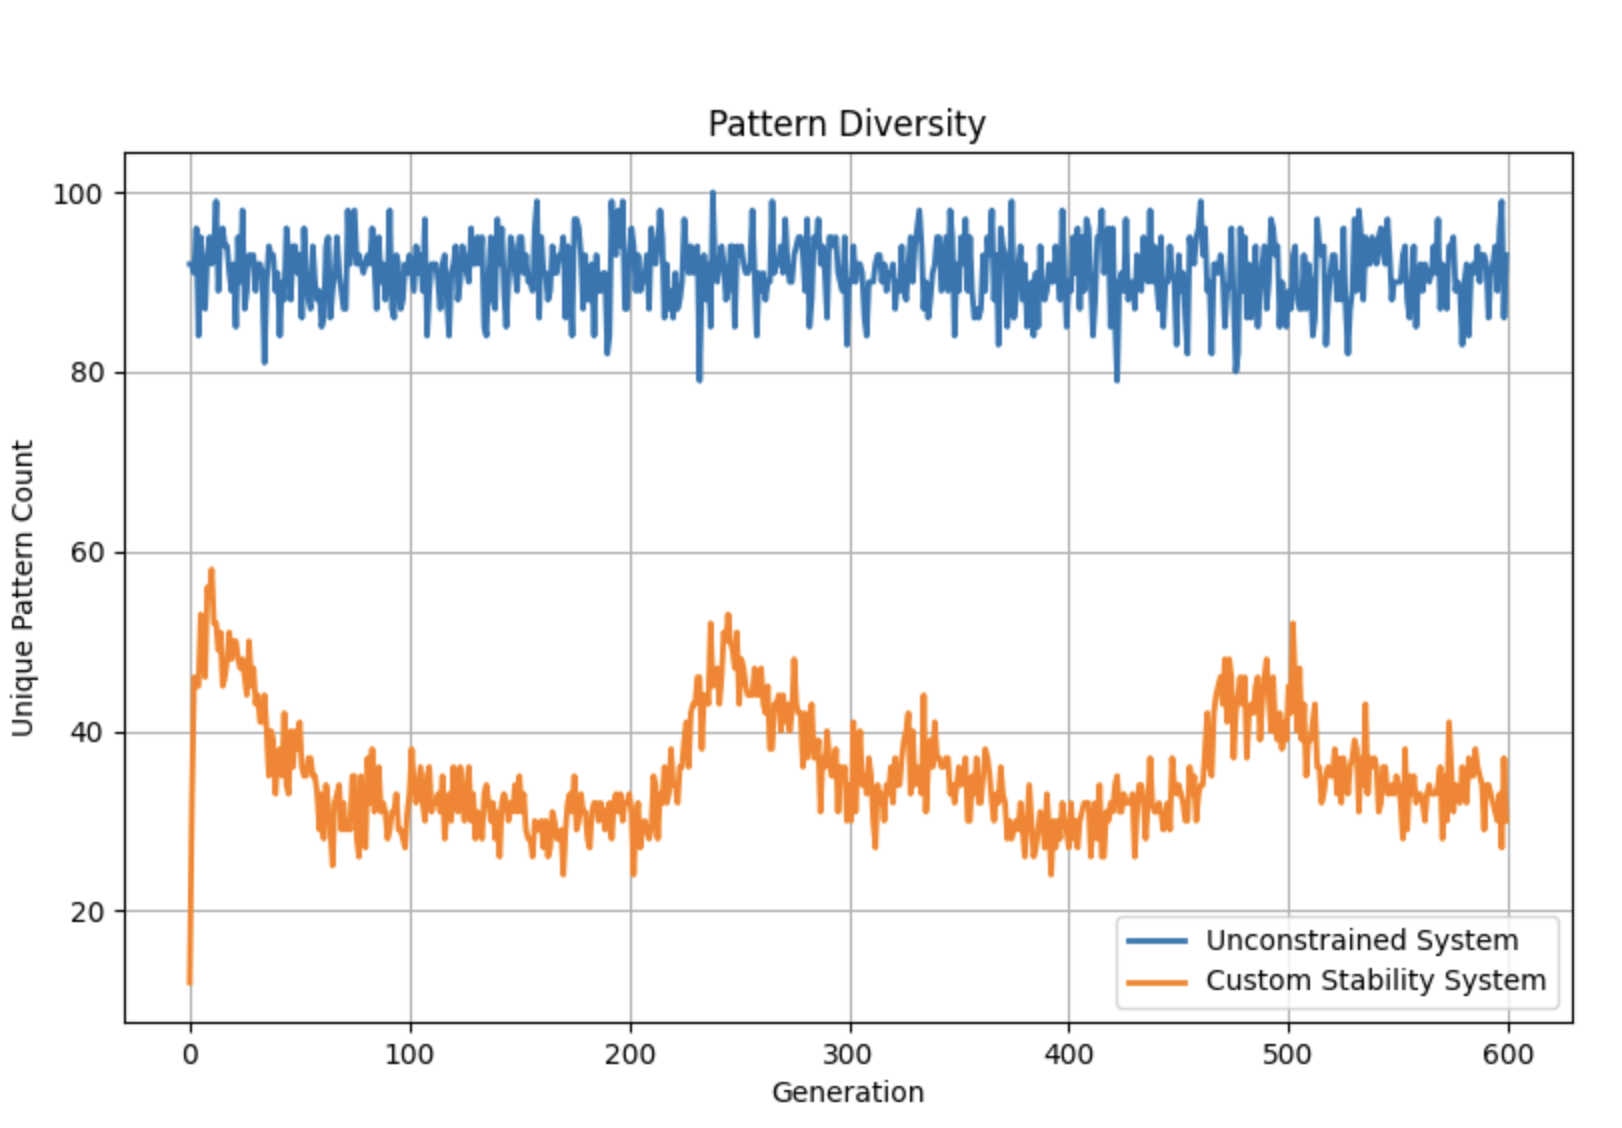
\includegraphics[width=0.75\textwidth]{SDA-concat-diversity.png}
    \caption{Pattern diversity in the concatenation-based SDA. Diversity oscillates in tandem with entropy, reflecting boom--bust cycles of synchronized motif turnover.}
    \label{fig:concat-diversity}
\end{figure}

\begin{figure}[H]
    \centering
    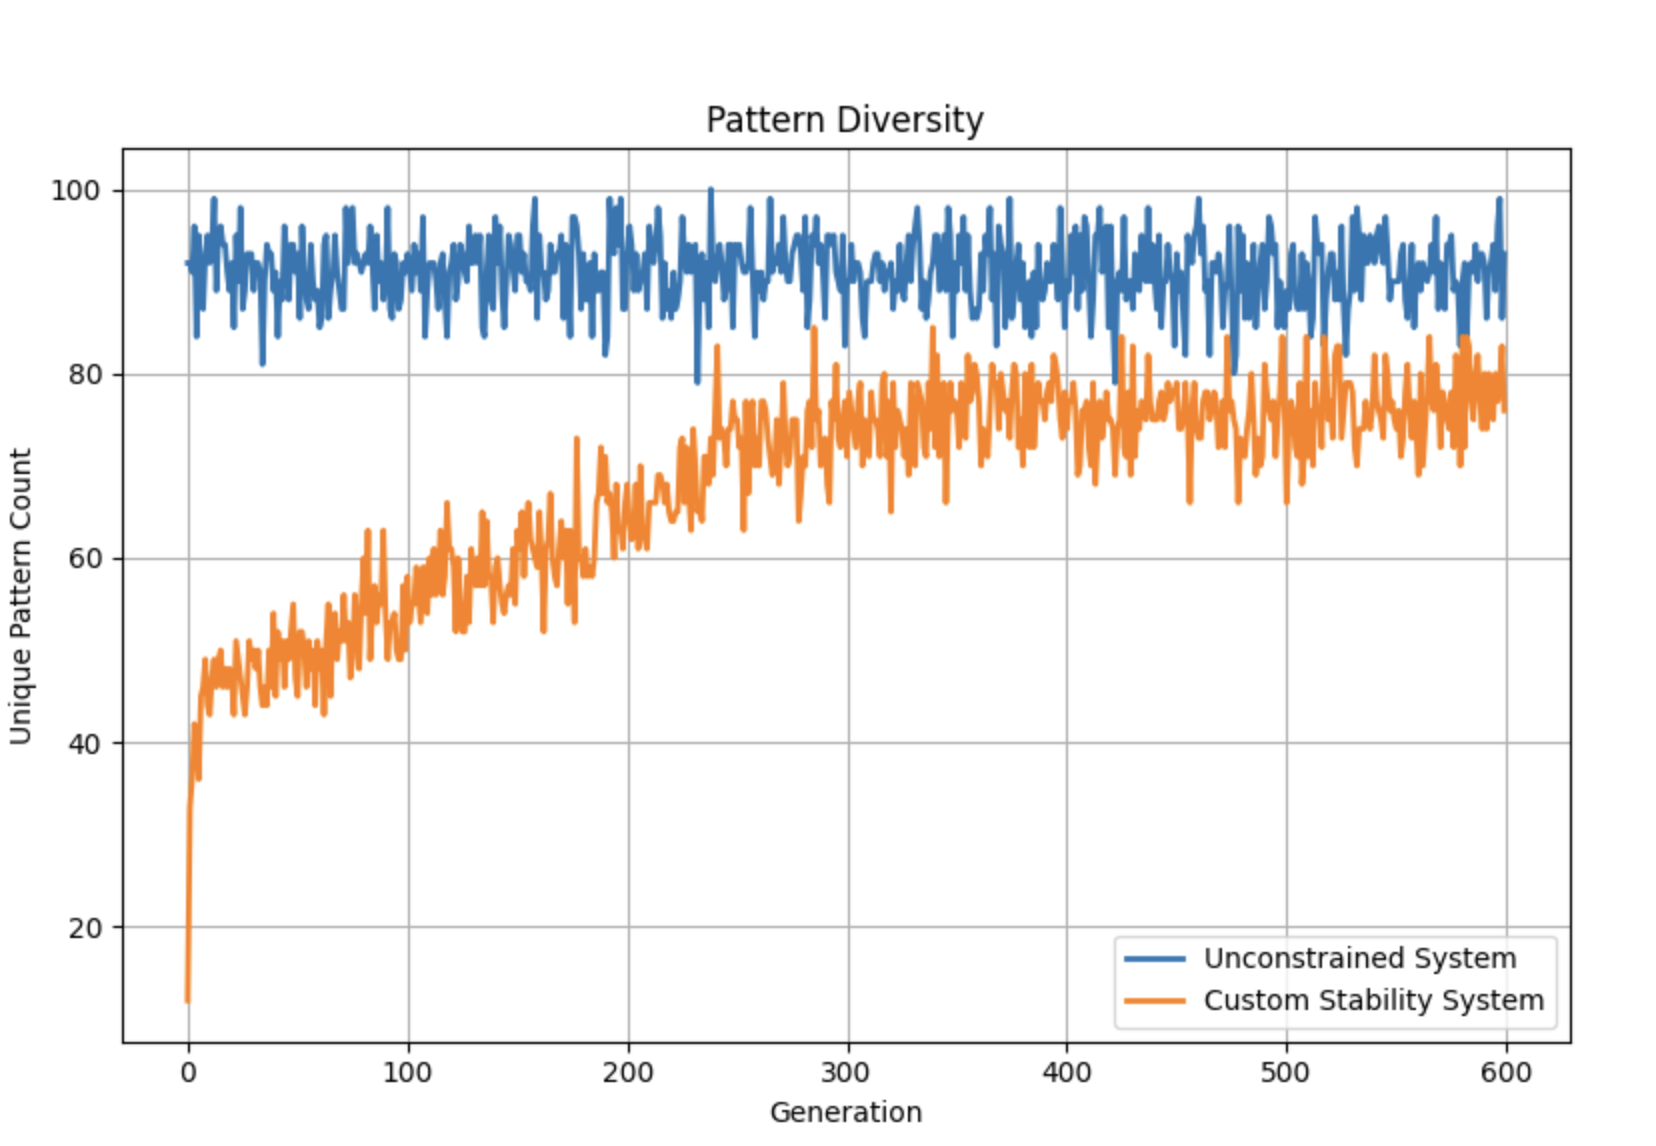
\includegraphics[width=0.75\textwidth]{SDA-GA-diversity.png}
    \caption{Pattern diversity in the recombination-based SDA/GA. Diversity steadily rises toward unconstrained levels, indicating continuous generation of low-frequency variants.}
    \label{fig:ga-diversity}
\end{figure}

The unique pattern diversity results in Figures~\ref{fig:concat-diversity} and~\ref{fig:ga-diversity} highlight the exploration--exploitation tradeoff. 
In concatenation-based SDA, exploration of pattern space is intermittent: 
diversity rises when base elements re-enter, then collapses as a dominant 
motif takes over, producing oscillatory boom--bust dynamics. In contrast, 
recombination-based SDA/GA sustains a broader exploration of the space, 
with diversity approaching unconstrained levels even though entropy 
collapses. Most of these additional patterns remain low-probability, but 
their presence shows that recombination and mutation inject continuous 
novelty. Thus, SDA/GA combines strong exploitation of stable motifs with 
ongoing exploration of alternatives---a hallmark of genetic algorithms---all 
emerging naturally without an explicit fitness function.


We also tested the effect of introducing low-probability, single-site mutations during recombination. 
These mutations serve as a simple model of stochastic perturbations such as copying errors or 
diffusion events. As expected, mutation did not qualitatively alter the dynamics: entropy still 
collapsed and high-stability motifs remained dominant. The principal effect was a modest increase 
in diversity, with rare variants persisting slightly longer. Importantly, mutation did not reintroduce 
oscillations into the GA case nor disrupt the overall reduction in entropy, confirming that the 
emergent selection mechanism is robust to stochastic noise.

\section{Genetic Algorithms and Natural Genetic Algorithms}

The study of genetic algorithms (GAs) has a long history in computer science and optimization. 
Holland’s foundational work \cite{holland1975adaptation} introduced the idea of using crossover, 
mutation, and selection to evolve solutions to computational problems. Later, Goldberg 
\cite{goldberg1989genetic} popularized and formalized GAs as practical optimization tools, 
particularly for engineering and combinatorial search. Building on this tradition, Koza 
\cite{koza1992genetic} extended the paradigm to genetic programming (GP), in which whole 
program trees rather than fixed-length strings evolve under crossover and mutation. GP has 
been especially influential in symbolic regression and in evolving nontrivial structures such 
as circuits, strategies, and controllers.

In all of these approaches, the defining feature of a GA or GP is that the \emph{fitness function} 
is externally specified by the programmer. The GA loop evaluates each candidate solution, assigns 
a fitness value, and uses that fitness to bias the sampling of parents. Whether the goal is 
minimizing error in a regression task or maximizing throughput in a design problem, the selective 
pressure is supplied by the problem designer.


By contrast, in a Stability-Driven Assembly (SDA) system the selection mechanism is not externally 
programmed but emerges intrinsically from persistence. Each pattern has a stability $S(p)$, 
which determines how long it remains in the population. Patterns with higher stability survive 
longer, become more frequent, and are therefore more likely to be sampled for further 
recombination. This effectively implements a roulette-wheel selection scheme without explicitly 
specifying one in the algorithm.

In simple string models, the stability function $S$ may be assigned by hand to highlight specific 
motifs, which makes the dynamics easy to visualize. However, in real-world contexts the stability 
function is determined by the environment itself. In chemistry, for example, molecular stability 
arises from thermodynamics, kinetics, and reaction constraints. In biology, environmental conditions 
determine whether a sequence or structure persists. Thus, while a traditional GA requires the 
programmer to provide an explicit fitness function, a natural GA---as instantiated by SDA---derives 
its fitness measure from the environment. This distinction is crucial for interpreting SDA not 
merely as an algorithmic metaphor but as a model of how nature itself performs search and selection.

Classical GA uses an explicit programmer-supplied fitness function $f$ to bias selection. 
In SDA, there is no explicit selection operator: each pattern $p$ receives a stability 
$S(p)$ that sets its expiration time $t_{\exp}(p)=t+S(p)$. Patterns with larger $S(p)$ 
persist longer and are therefore sampled more often for recombination, yielding 
fitness-proportional selection \emph{in expectation} without computing $f$. 
For toy strings, $S$ may be assigned by design; for realistic chemistry, $S$ is determined 
by the environment (valence/duet–octet satisfaction, sterics, thermodynamics, kinetics, 
reactor residence time). Thus, SDA \emph{builds fitness into persistence}, whereas GA 
\emph{supplies fitness explicitly}.

\section{Application to Organic Chemistry}

The abstract SDA/GA framework can be instantiated in chemical symbol space to model 
the spontaneous evolution of molecular populations. In this setting, the base elements 
$E$ are drawn from the atomic alphabet (C, O, N, H, etc.), and the interaction operator 
$\oplus$ is instantiated as recombination and mutation of molecular fragments. 

Genetic algorithms and genetic programming have long been applied in chemistry and 
cheminformatics, particularly for de novo molecular design and drug discovery 
\cite{brown2004ga,lewis1998gp,jensen2019ga,yoshikawa2018ga}. These approaches typically 
represent molecules as graphs or strings and apply crossover and mutation operators 
guided by an externally defined fitness function, such as binding affinity, 
drug-likeness, or synthetic accessibility. Fink and Reymond’s construction of the 
GDB-11 database \cite{fink2007gdb11} demonstrated the sheer size of chemically valid 
search space, generating over 26 million molecules with up to eleven atoms and over 
110 million stereoisomers. Yet only a minute fraction of these compounds occur in 
public databases, underscoring both the vastness of chemical possibility and the 
impracticality of uniform or ergodic search. This observation motivates the use of 
search strategies that inherently bias exploration toward persistent and chemically 
stable motifs. Whereas traditional GA/GP methods rely on explicit, human-specified 
fitness functions to impose such bias, the SDA/GA framework does so intrinsically by 
embedding stability into persistence, allowing selection pressure to emerge directly 
from environmental constraints such as valence rules, steric feasibility, and 
thermodynamics.

It is important to emphasize that the present work is not aimed at drug discovery 
or molecular optimization applications, which have been the traditional focus of 
genetic algorithms and genetic programming in chemistry. Instead, our goal is 
conceptual: to hypothesize how nature itself may have acted as a “natural genetic 
algorithm,” using stability-driven persistence as the implicit fitness function to 
non-ergodically explore the astronomical chemical space revealed by studies such 
as GDB-11. Within this perspective, the emergence of a biosphere can be viewed as 
the outcome of stability-biased sampling: persistent motifs accumulate, dominate, 
and recombine, gradually transforming an unconstrained chemical universe into a 
structured, evolving system.


\subsection{Patterns as Molecules}
Patterns correspond to molecules represented in SMILES notation. Recombination is implemented 
using BRICS fragmentation and reassembly, ensuring that new molecules respect basic valence 
rules and avoid chemically implausible bonds. Mutation is modeled as single-site perturbations, 
analogous to copying errors or diffusion-induced reactions, again constrained by chemical 
plausibility.

\subsection{Stability as Persistence}
In the chemical domain, the stability function $S(p)$ is determined by the environment rather 
than by the algorithm designer. For organic molecules, persistence may reflect compliance with 
the octet rule, avoidance of strained substructures, thermodynamic feasibility, or kinetic 
barriers to decay. In practice, we operationalize $S(p)$ using fast cheminformatics heuristics 
(RDKit valence checks, BRICS rules) that enforce plausible structures. More detailed models 
could extend $S(p)$ to incorporate semiempirical energy estimates or experimentally derived 
lifetimes.

\subsection{Simulation Examples}
Applying the SDA/GA procedure to organic fragments yields results analogous to the string 
experiments. High-stability motifs dominate the population, while recombination continually 
generates low-frequency variants, maintaining a fat-tailed distribution of molecules. Entropy 
collapses as selection pressure drives convergence, yet diversity remains higher under 
recombination than under concatenation, reflecting ongoing exploration of chemical space. 
These dynamics mirror nature’s own exploration of chemical possibility: vast combinatorial 
search space is sampled non-ergodically, biased toward persistent structures.

\subsection{Interpretation}
This chemical instantiation highlights the central claim of SDA: selection emerges not from 
an externally defined fitness function, but from persistence. In GA terms, fitness is 
\emph{calculated} by the environment. In practice, octet completion, steric constraints, and 
reaction kinetics determine which molecules last long enough to be sampled again. Thus, the 
SDA/GA framework offers a naturalistic model of molecular evolution, one that unifies symbolic 
cheminformatics with dynamical systems principles.

\section{Chemical SDA/GA Simulation}

\subsection{Methods}

To extend the symbolic SDA/GA framework into the chemical domain, we reused the same minimal simulation loop with only two modifications. First, symbolic string elements were replaced with SMILES fragments drawn from a small set of base compounds (e.g., \texttt{C}, \texttt{CC}, \texttt{O}, \texttt{CO}, etc.), representing a rudimentary pool of prebiotic building blocks. Second, instead of assigning fixed stability values, we introduced a callable stability function $S(p)$ that estimates the persistence of a compound from molecular features. For demonstration purposes, this was implemented as a function of heavy atom count with heuristic boosts for chemically plausible motifs such as carboxylates, esters, and amides. In this formulation, fitness is not supplied externally, but arises from chemical plausibility as encoded in stability, thereby aligning with the SDA principle that selection emerges from persistence rather than externally imposed objectives.  

All other aspects of the algorithm were left unchanged. As in the symbolic case, base fragments were replenished each generation, new compounds were formed through recombination and mutation using BRICS rules, and expiration times were assigned according to the stability function. This allows the chemical simulation to be understood as a natural extension of symbolic SDA, with only minimal changes distinguishing abstract informational dynamics from physical chemical dynamics.  

\subsection{Results}

We ran simulations for 600 generations with 100 interactions per generation and replenishment rate of three. Several metrics were collected to characterize the evolutionary dynamics of the chemical system.  

\begin{figure}[H]
    \centering
    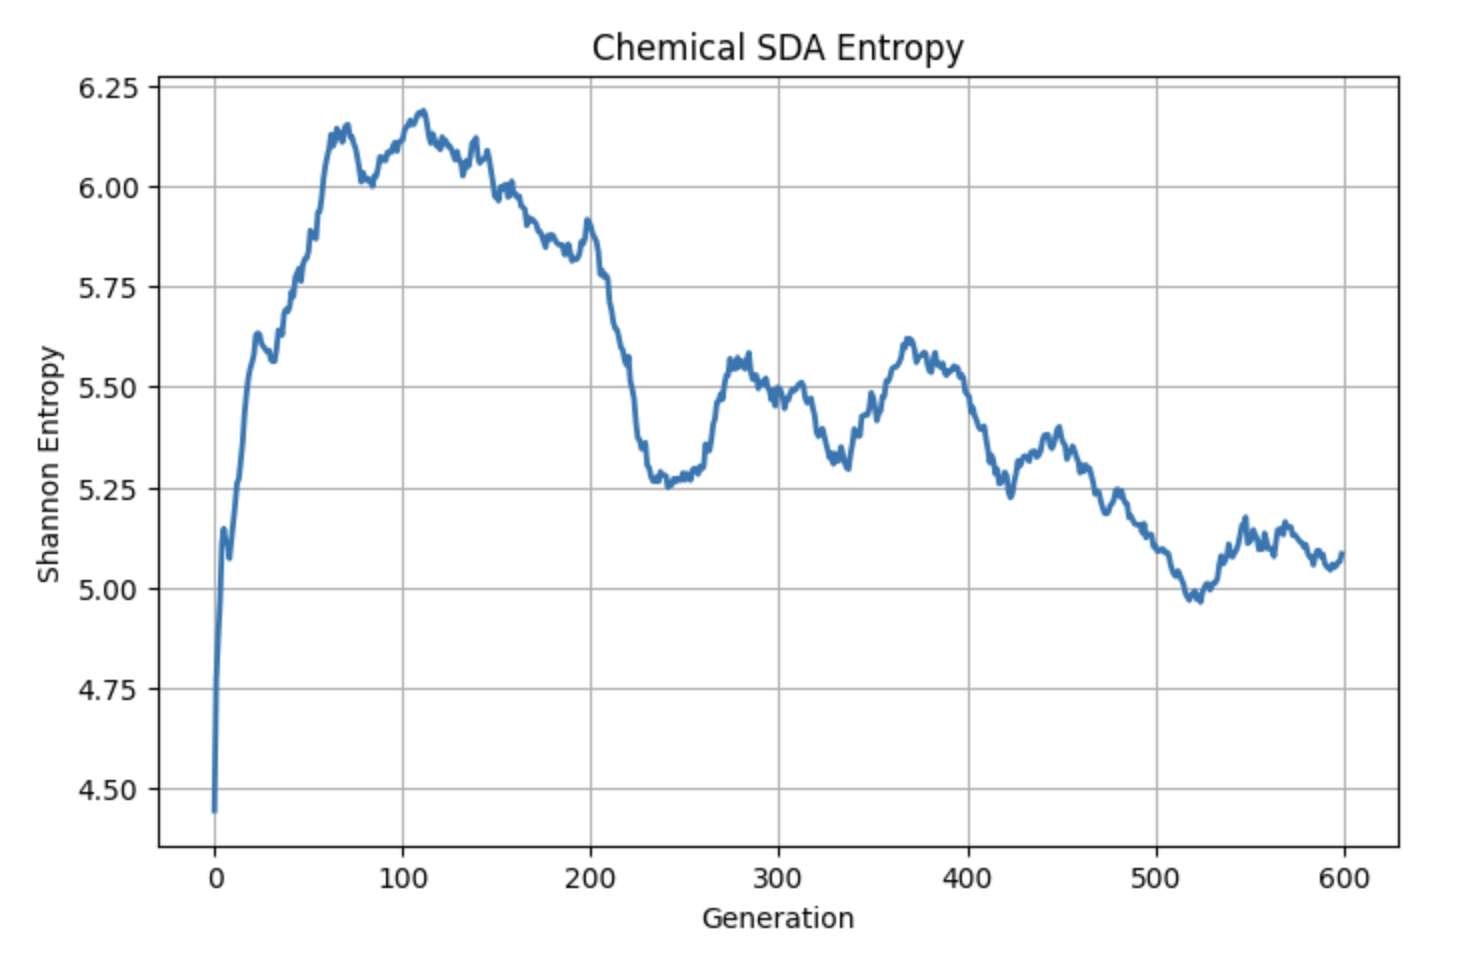
\includegraphics[width=0.7\textwidth]{SDA-chem-entropy.png}
    \caption{Shannon entropy of the chemical SDA population over 600 generations. Entropy rises sharply as diversity expands, then exhibits oscillations reflecting alternating phases of order and disorder as dominant motifs emerge and collapse.}
    \label{fig:chem-entropy}
\end{figure}

Figure~\ref{fig:chem-entropy} shows the entropy trajectory of the chemical population. Entropy initially rises rapidly as new compounds are discovered, then exhibits a pattern of oscillations rather than monotonic decay. These oscillations are consistent with the boom–bust cycles seen in symbolic SDA runs, in which clusters of stable patterns temporarily dominate before being displaced by alternative structures. The persistence of oscillations indicates that stability-driven selection is sufficient to generate long-lived cycles of order and disorder.  

\begin{figure}[H]
    \centering
    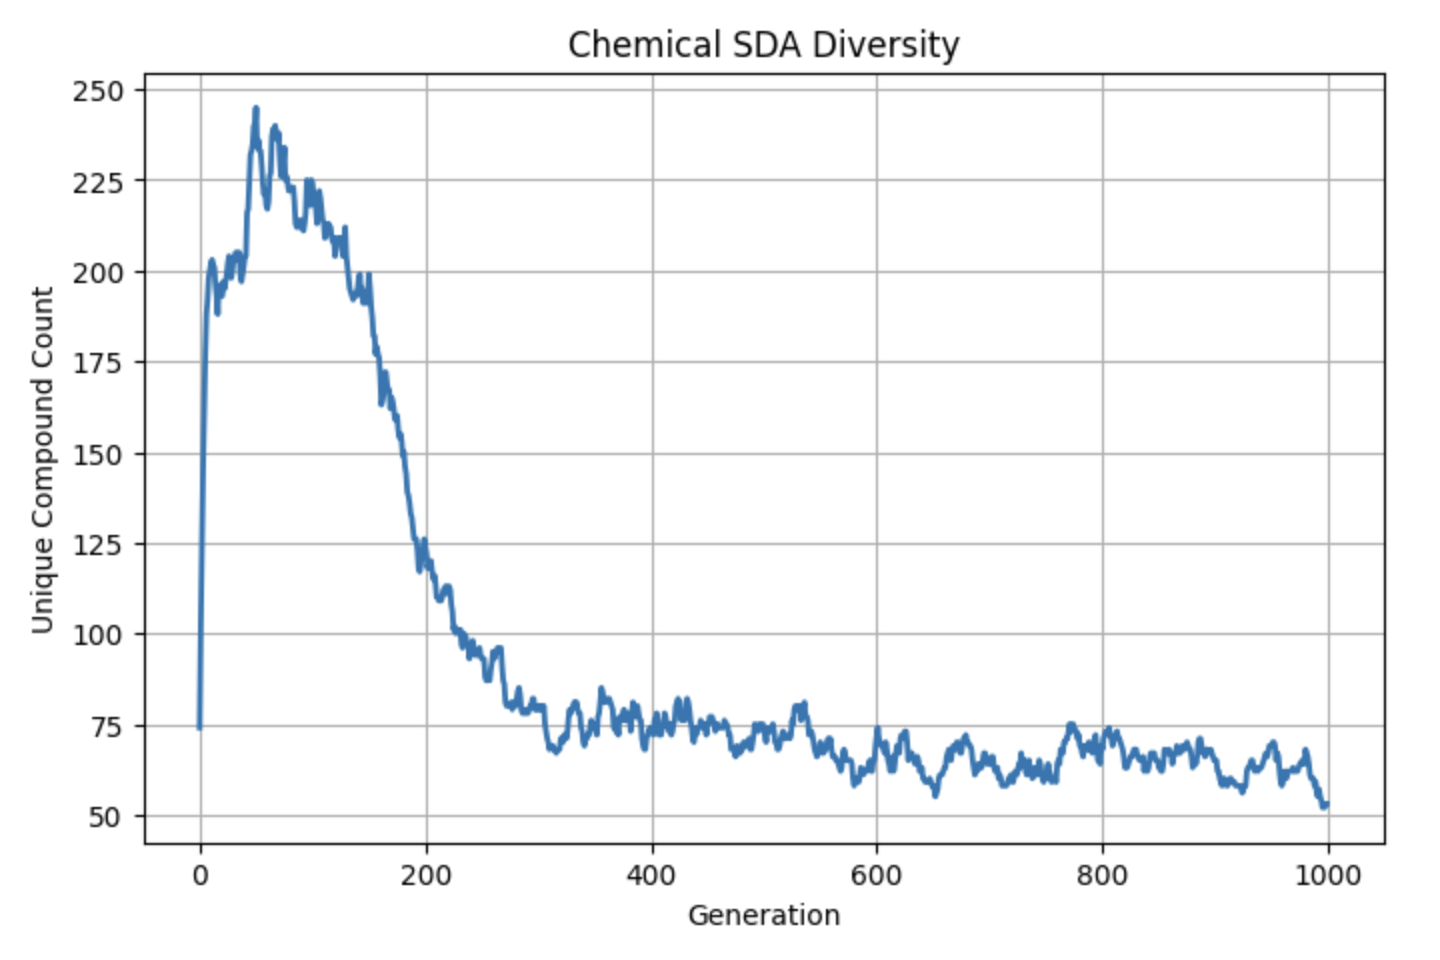
\includegraphics[width=0.7\textwidth]{SDA-chem-diversity.png}
    \caption{Unique compound count over time. Diversity rises steeply in early generations and stabilizes around 100–140 species, with oscillations that closely track entropy fluctuations.}
    \label{fig:chem-diversity}
\end{figure}

The diversity of unique compounds, shown in Figure~\ref{fig:chem-diversity}, follows a similar trajectory. After a rapid increase in early generations, the number of distinct compounds stabilizes at around 100–140, fluctuating in tandem with entropy. This parallelism reinforces the interpretation that entropy oscillations correspond to turnover in chemical diversity, where new motifs periodically displace previously dominant ones.  

\begin{figure}[H]
    \centering
    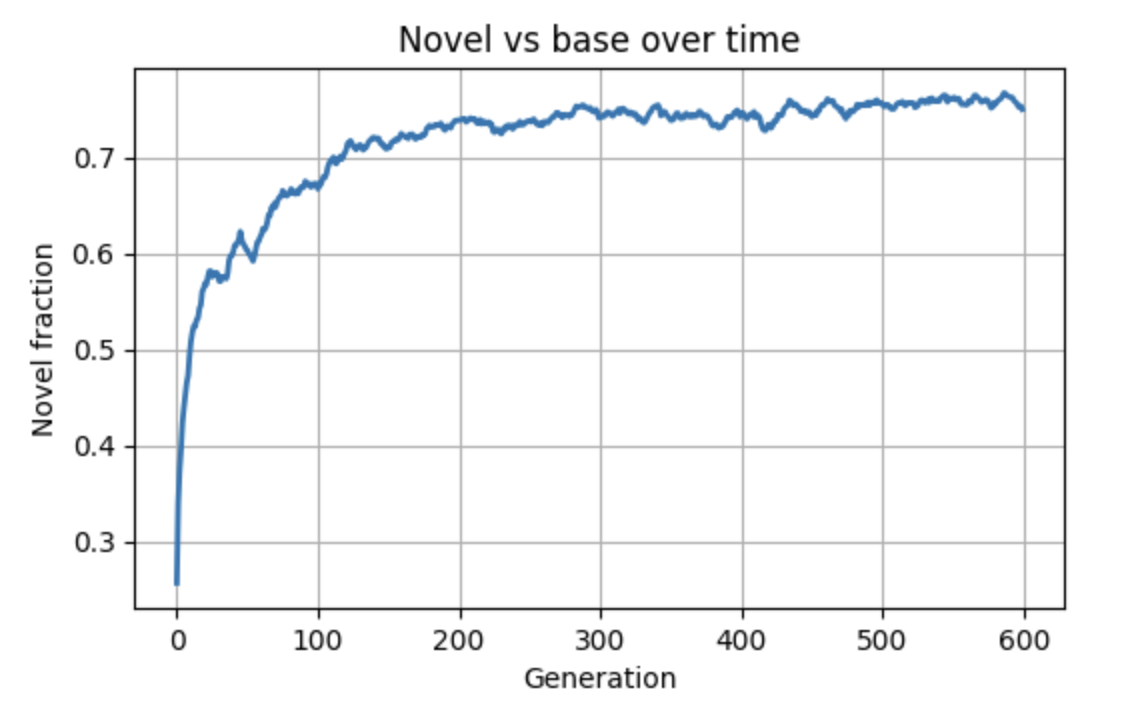
\includegraphics[width=0.7\textwidth]{SDA-chem-novel.png}
    \caption{Fraction of novel compounds (not in the initial fragment pool) over time. By generation 600, approximately 75\% of the population consists of novel compounds, demonstrating continuous innovation through recombination and mutation.}
    \label{fig:chem-novel}
\end{figure}

Figure~\ref{fig:chem-novel} quantifies the share of novel compounds relative to the base fragment pool. The fraction of novel structures rises steadily and plateaus near 75\%, showing that recombination and mutation efficiently explore new regions of chemical space. The persistence of this fraction demonstrates that novelty is not transient but sustained across generations, as stable new motifs accumulate and contribute to ongoing evolutionary dynamics.  

\begin{figure}[H]
    \centering
    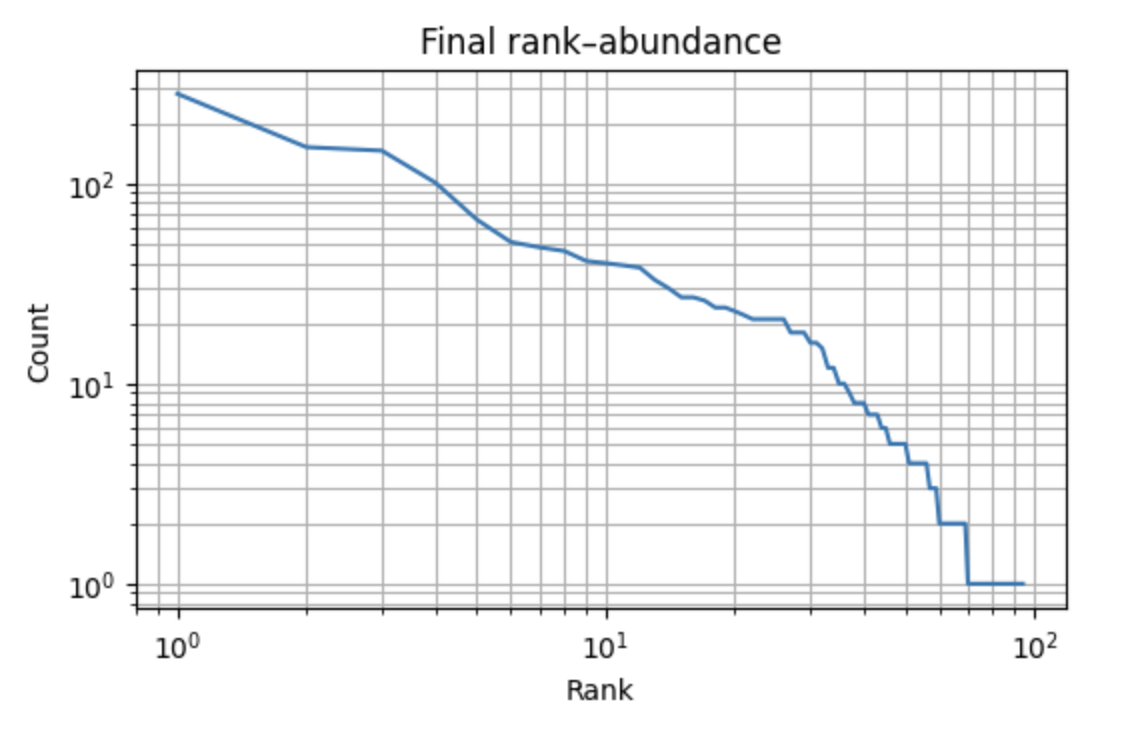
\includegraphics[width=0.7\textwidth]{SDA-chem-rank.png}
    \caption{Rank–abundance distribution of compounds in the final population (log–log scale). The heavy-tailed form, with a few highly abundant compounds and many rare ones, resembles ecological species-abundance distributions.}
    \label{fig:chem-rank}
\end{figure}

The rank–abundance distribution in Figure~\ref{fig:chem-rank} shows a heavy-tailed profile typical of complex adaptive systems. A few highly abundant compounds dominate, while many rare ones persist at low frequency. This mirrors species-abundance curves in ecology, further underscoring the natural GA-like properties of SDA when applied to chemical space.  

\begin{figure}[H]
    \centering
    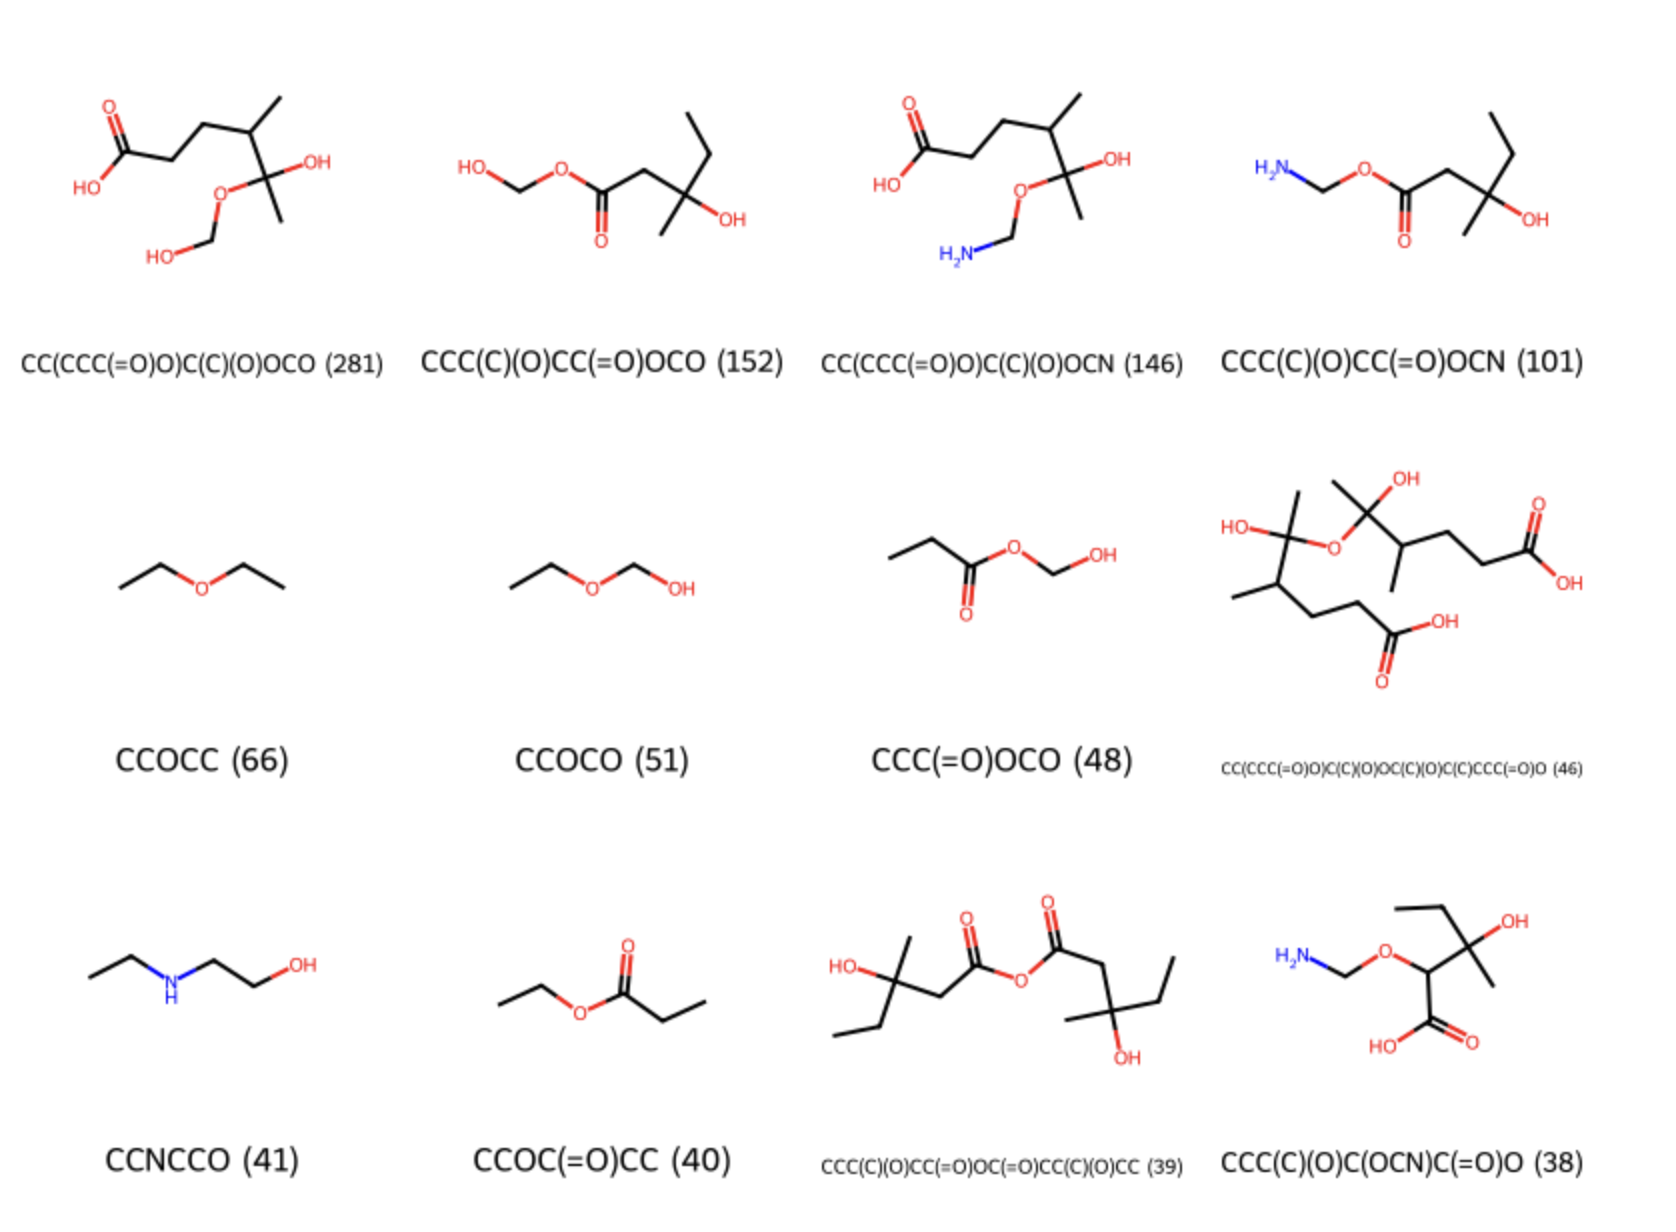
\includegraphics[width=0.9\textwidth]{SDA-chem-compounds.png}
    \caption{Representative structures of the twelve most abundant compounds at the end of the simulation. Compounds exhibit chemically plausible motifs such as esters, hydroxyl groups, and amide-like linkages, despite the use of a simple heuristic stability function.}
    \label{fig:chem-compounds}
\end{figure}

The most persistent compounds are depicted in Figure~\ref{fig:chem-compounds}. Even though the stability function was a simplified proxy, many of the top-ranking compounds exhibit motifs consistent with chemical plausibility, including esters, hydroxylated carbons, and amide-like linkages. Their emergence highlights that stability-driven persistence alone can generate complex and structured chemistry from a small base set.  

\begin{figure}[H]
    \centering
    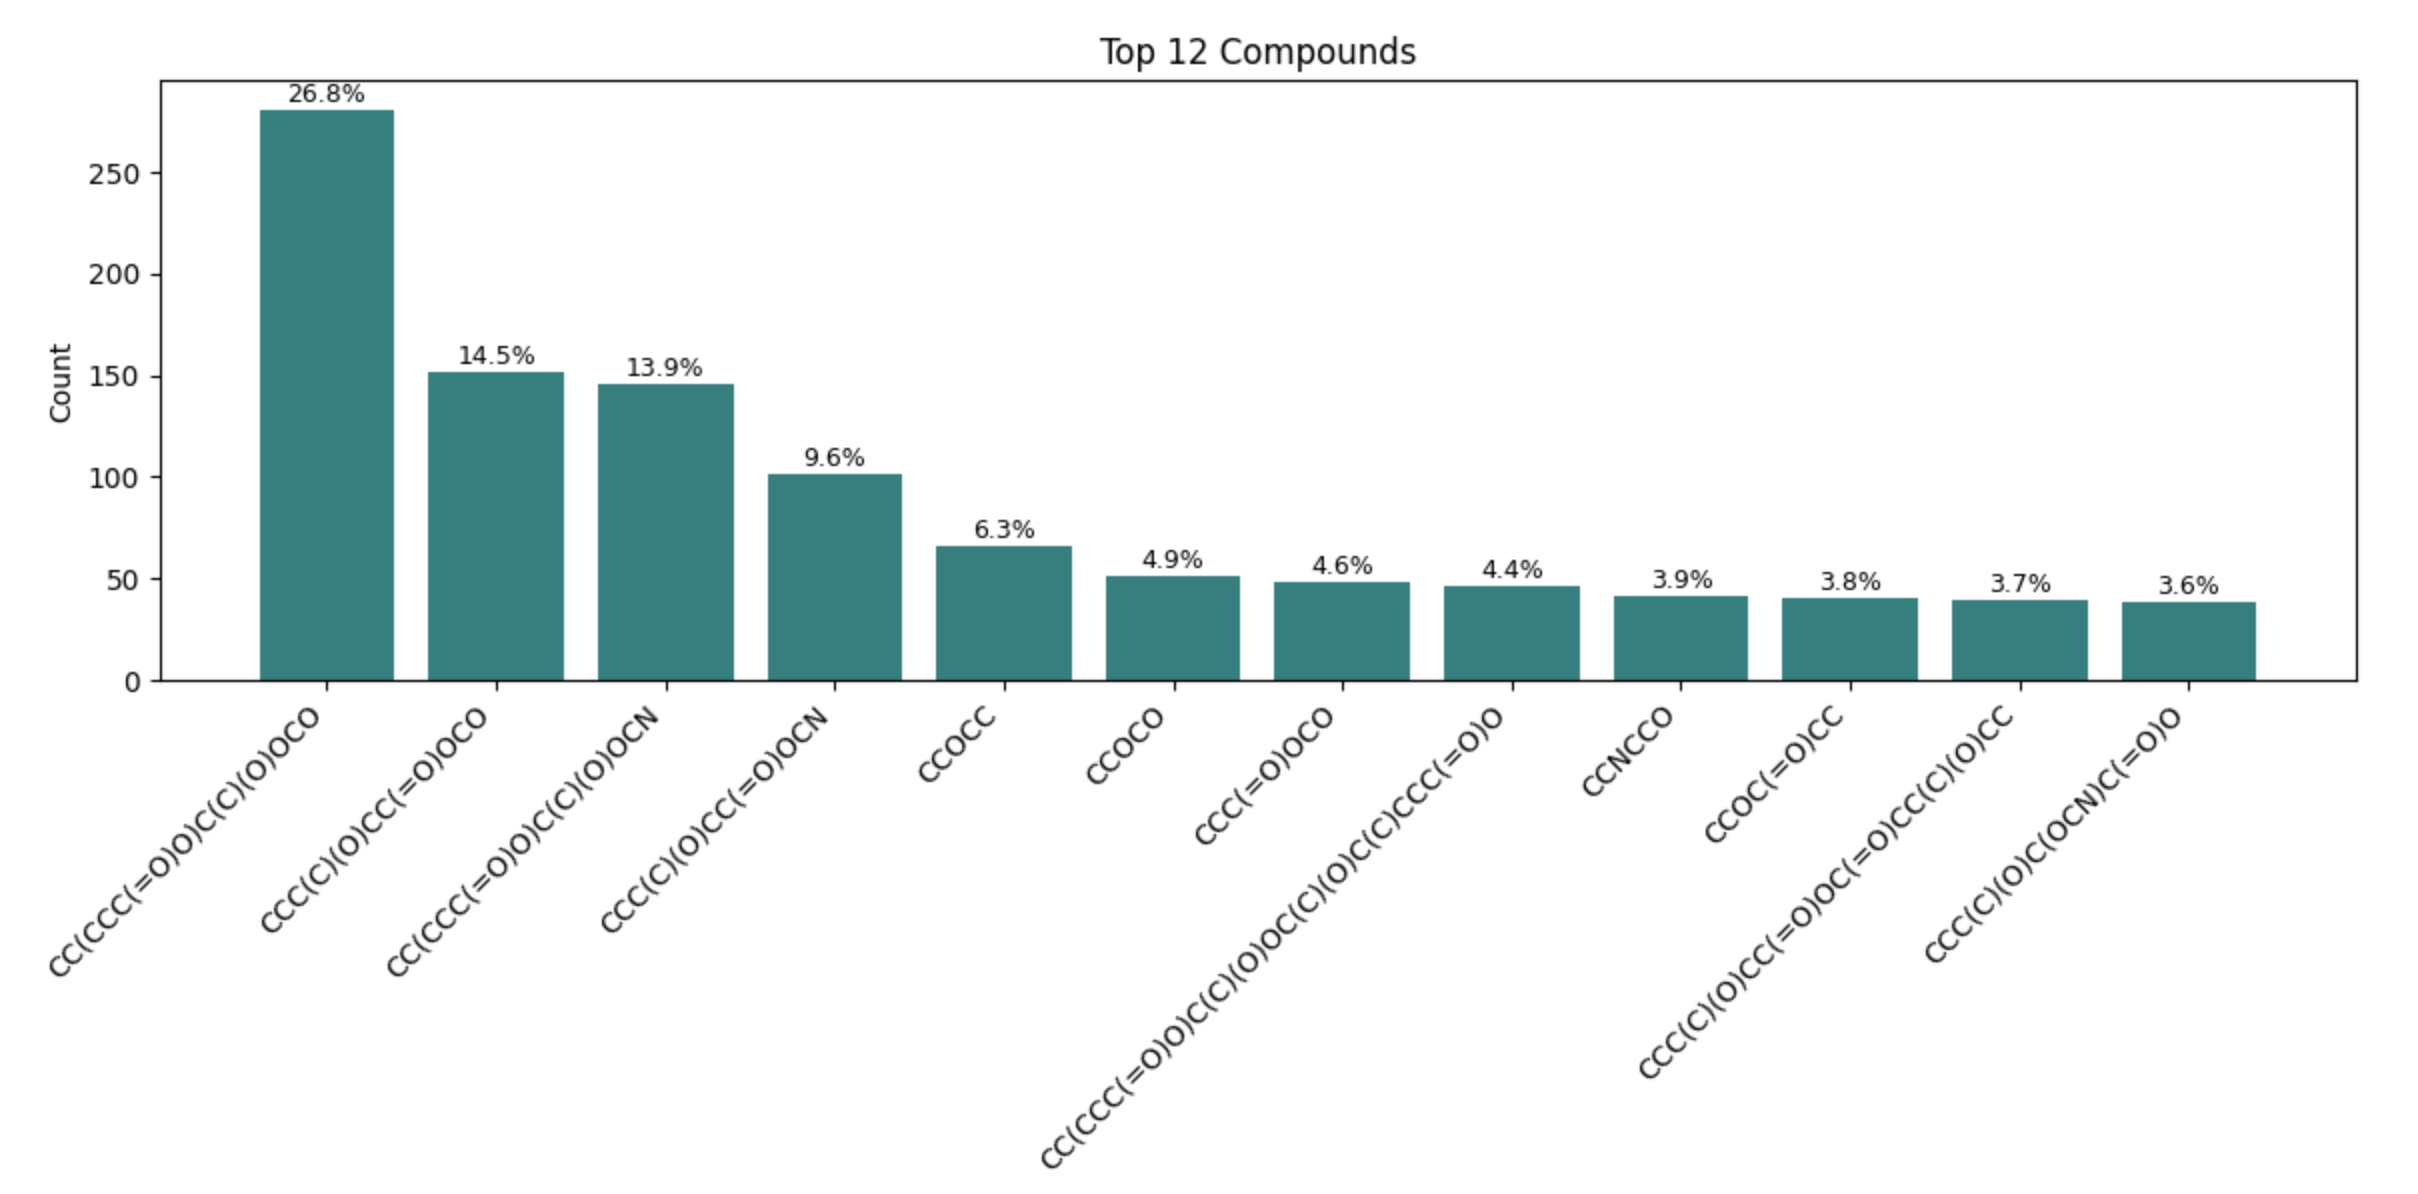
\includegraphics[width=0.9\textwidth]{SDA-chem-compound-hist.png}
    \caption{Histogram of the twelve most frequent compounds, expressed both in counts and relative percentages. A few compounds achieve dominance while others remain at intermediate frequencies, producing a heterogeneous but structured population.}
    \label{fig:chem-compound-hist}
\end{figure}

The histogram in Figure~\ref{fig:chem-compound-hist} further illustrates the dominance of a small number of compounds. The leading compound comprises nearly 27\% of the population, with subsequent compounds contributing smaller but still significant shares. This uneven distribution aligns with the rank–abundance profile and demonstrates how stability-driven selection naturally produces heterogeneity in chemical ecosystems.  

\subsection{Interpretation}

Taken together, these results demonstrate that the SDA framework, when instantiated with chemical fragments, behaves as a natural genetic algorithm. At the symbolic level, the system consists of nothing more than recombination, mutation, replenishment, and stability-driven expiration. Yet when applied to chemical fragments, these same operations generate persistent novelty, heavy-tailed abundance distributions, and oscillatory dynamics of entropy and diversity.  

Crucially, fitness is not an externally imposed function, as in conventional GAs, but emerges from the persistence of chemically plausible structures. In the symbolic case this was pre-specified through a lookup table of stability values; in the chemical case it is calculated implicitly by the environment through the stability function. This distinction highlights the dual nature of SDA: it is simultaneously a model of symbolic information dynamics and a plausible mechanistic account of how chemistry could self-organize into increasingly complex structures, ultimately giving rise to a biosphere.  



\section{Open-Endedness and Computation}

\section{From Chemistry to Evolution}

\section{Implications}
\subsection{Origins of Life}
\subsection{Astrobiology}
\subsection{Philosophy of Evolution}
\subsection{Echoes in Biology}

\section{Conclusion}


\funding{This research received no external funding}

\institutionalreview{Not applicable}

\informedconsent{Not applicable}

\dataavailability{Not applicable} 

\acknowledgments{}

\conflictsofinterest{The author declares no conflicts of interest} 

\begin{adjustwidth}{-\extralength}{0cm}
%\printendnotes[custom] % Un-comment to print a list of endnotes

\reftitle{References}



% Please provide either the correct journal abbreviation (e.g. according to the “List of Title Word Abbreviations” http://www.issn.org/services/online-services/access-to-the-ltwa/) or the full name of the journal.
% Citations and References in Supplementary files are permitted provided that they also appear in the reference list here. 

%=====================================
% References, variant A: external bibliography
%=====================================
% \bibliography{your_external_BibTeX_file}

%=====================================
% References, variant B: internal bibliography
%=====================================

% ACS format
\isAPAandChicago{}{%
\begin{thebibliography}{999}
% Reference 1

\bibitem{adler_sda}
Adler, D.
\textit{Stability-Driven Assembly Theory}.
SSRN Preprint, 2025. Available at: \url{https://dx.doi.org/10.2139/ssrn.5203036}

\bibitem{holland1975adaptation}
Holland, J.H. \textit{Adaptation in Natural and Artificial Systems}; University of Michigan Press: Ann Arbor, MI, USA, 1975.

\bibitem{goldberg1989genetic}
Goldberg, D.E. \textit{Genetic Algorithms in Search, Optimization, and Machine Learning}; Addison-Wesley: Boston, MA, USA, 1989.

\bibitem{koza1992genetic}
Koza, J. R.
\textit{Genetic Programming: On the Programming of Computers by Means of Natural Selection}.
MIT Press, Cambridge, MA, USA, 1992.

\bibitem{fink2007gdb11}
Fink, T.; Reymond, J.-L.
\textit{Virtual exploration of the chemical universe up to 11 atoms of C, N, O, F:
Assembly of 26.4 million structures (GDB-11).}
J. Chem. Inf. Model. 2007, 47, 342--353.

\bibitem{brown2004ga}
Brown, N.; McKay, B.; Gilardoni, F.; Gasteiger, J.
\textit{A graph-based genetic algorithm and its application to the multiobjective
evolution of median molecules.}
J. Chem. Inf. Comput. Sci. 2004, 44, 1079--1087.

\bibitem{lewis1998gp}
Lewis, R. A.
\textit{Genetic programming as a model for drug design.}
J. Chem. Inf. Comput. Sci. 1998, 38, 651--657.

\bibitem{jensen2019ga}
Jensen, J. H.
\textit{A graph-based genetic algorithm and generative model/GA hybrid for molecular discovery.}
Chem. Sci. 2019, 10, 3567--3572.

\bibitem{yoshikawa2018ga}
Yoshikawa, N.; Terayama, K.; Sumita, M.; Homma, T.; Oono, K.; Tsuda, K.
\textit{Population-based de novo molecule generation, using grammatical evolution.}
Chem. Lett. 2018, 47, 1431--1434.


\end{thebibliography}
}



% If authors have biography, please use the format below
%\section*{Short Biography of Authors}
%\bio
%{\raisebox{-0.35cm}{\includegraphics[width=3.5cm,height=5.3cm,clip,keepaspectratio]{Definitions/author1.pdf}}}
%{\textbf{Firstname Lastname} Biography of first author}
%
%\bio
%{\raisebox{-0.35cm}{\includegraphics[width=3.5cm,height=5.3cm,clip,keepaspectratio]{Definitions/author2.jpg}}}
%{\textbf{Firstname Lastname} Biography of second author}

% For the MDPI journals use author-date citation, please follow the formatting guidelines on http://www.mdpi.com/authors/references
% To cite two works by the same author: \citeauthor{ref-journal-1a} (\citeyear{ref-journal-1a}, \citeyear{ref-journal-1b}). This produces: Whittaker (1967, 1975)
% To cite two works by the same author with specific pages: \citeauthor{ref-journal-3a} (\citeyear{ref-journal-3a}, p. 328; \citeyear{ref-journal-3b}, p.475). This produces: Wong (1999, p. 328; 2000, p. 475)

%%%%%%%%%%%%%%%%%%%%%%%%%%%%%%%%%%%%%%%%%%
%% for journal Sci
%\reviewreports{\\
%Reviewer 1 comments and authors’ response\\
%Reviewer 2 comments and authors’ response\\
%Reviewer 3 comments and authors’ response
%}
%%%%%%%%%%%%%%%%%%%%%%%%%%%%%%%%%%%%%%%%%%
\PublishersNote{}
%\isPreprints{} % If the paper is ``preprints'', please uncomment this parenthesis.
\end{document}

